\documentclass[a4paper,14pt]{extarticle}
\usepackage{../../tex-shared/report-layout}

\renewcommand{\mylabnumber}{4}
\renewcommand{\mylabtitle}{Кластерный анализ. Основные этапы и задачи кластерного анализа данных}
\renewcommand{\mysubject}{Интеллектуальный анализ данных}
\renewcommand{\mylecturer}{Сырых О.А.}

\begin{document}
\begin{titlepage}
    
    \thispagestyle{empty}
    
    \begin{center}
        
        Министерство науки и Высшего образования Российской Федерации \\
        Севастопольский государственный университет \\
        Кафедра ИС
        
        \vfill

        Отчет \\
        по лабораторной работе №\mylabnumber \\
        \enquote{\mylabtitle} \\
        по дисциплине \\
        \enquote{\MakeTextUppercase{\mysubject}}

    \end{center}

    \vspace{1cm}

    \noindent\hspace{7.5cm} Выполнил студент группы ИС/б-17-2-о \\
    \null\hspace{7.5cm} Горбенко К. Н. \\
    \null\hspace{7.5cm} Проверил \\
    \null\hspace{7.5cm} \mylecturer

    \vfill

    \begin{center}
        Севастополь \\
        \the\year{}
    \end{center}

\end{titlepage}

\section{Цель работы}
\begin{itemize}
    \item закрепить теоретические знания и приобрести практические навыки в
          проведении кластерного анализа по экспериментальным данным;
    \item исследовать возможности языка R для проведения кластерного анализа.
\end{itemize}

\section{Задание на работу}
\begin{enumerate}
    \item Создать файл с исходными данными.
    \item Провести кластерный анализ экспериментальных данных.
    \item Проведя процедуру кластеризации несколько раз при различных значениях
          числа кластеров (от 2-х до 10 кластеров), необходимо выбрать лучшую
          группировку в смысле критерия минимума отношений средних внутри
          кластерных и меж кластерных расстояний. Полученные результаты оформите
          в виде таблицы. Изобразить графически значения данного показателя
          качества классификации. Для этого построить диаграмму, на которой по
          оси Х – количество кластеров, по оси Y – значения показателя J.
\end{enumerate}

\section{Ход работы}
\subsection{Кластерный анализ}
Выполним иерархический кластерный анализ. Загрузим данные о количестве арестов в
США. Для этого воспользуемся известным набором данных из R, название которого
\enquote{USArrests}.

\begin{figure}[H]
    \centering
    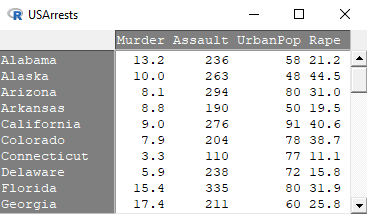
\includegraphics[width=.6\linewidth]{data-set}
    \caption{Загруженные данные}
    \label{fig:data-set}
\end{figure}

\begin{itemize}
    \item murder - количество задержаний за убийство;
    \item assault - количество задержаний за нападение;
    \item rape - количество задержаний за изнасилование;
    \item upban pop - процент городского населения.
\end{itemize}

Функция кластерного анализа в R:

\code{kmeans(x, centers, iter.шах=10, nstart=1,\\algorithm=c("Hartigan-Wong", "Lloyd", "Forgy", "MacQueen"))}

Выполним разбиение на два кластера по переменным \enquote{Количество убийств} и
\enquote{Количество нападений}. Результат разбиения изображен на рисунке
\ref{fig:2-clusters-graph}.

\begin{figure}[H]
    \centering
    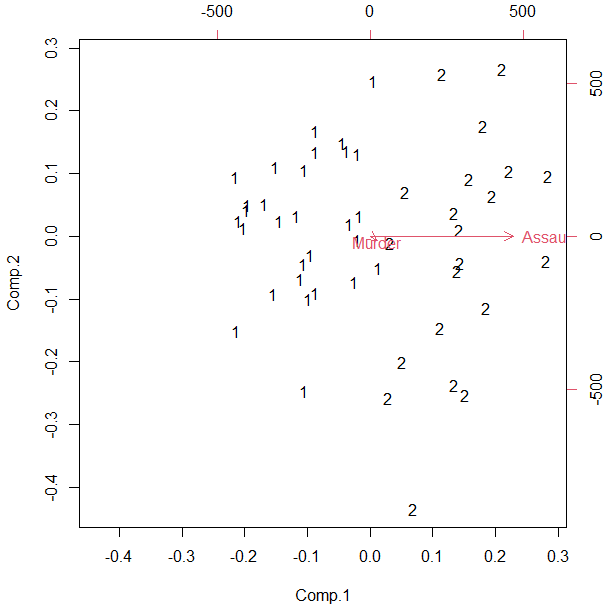
\includegraphics[width=.5\linewidth]{2-clusters-graph}
    \caption{Разбиение данных на 2 кластера}
    \label{fig:2-clusters-graph}
\end{figure}

Результаты разбиение представлены на рисунке \ref{fig:2-clusters-R}.

\begin{figure}[H]
    \centering
    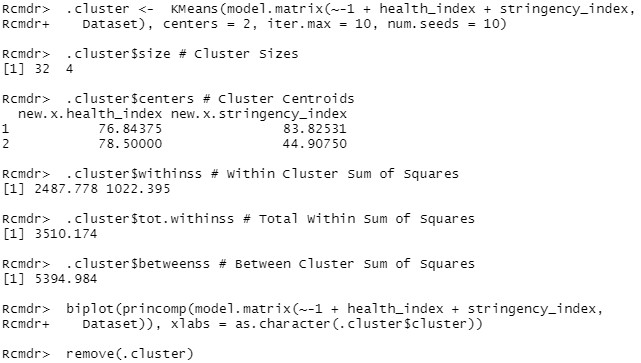
\includegraphics[width=.8\linewidth]{2-clusters-R}
    \caption{Результаты разбиения}
    \label{fig:2-clusters-R}
\end{figure}

\begin{itemize}
    \item первый кластер содержит 29 элементов, второй – 21;
    \item сумма квадратов расстояний внутри кластера: 1 – 47963, 2 – 35741;
    \item общая сумма квадратов расстояний внутри кластеров: 83705;
    \item сумма квадратов расстояний между кластерами – 257537.
\end{itemize}

Для выбора лучшей группировки в смысле критерия минимума отношений средних
внутри кластерных и меж кластерных расстояний было проведено деление на 3 – 10
кластеров и заполнена таблица в MS Excel.

\begin{figure}[H]
    \centering
    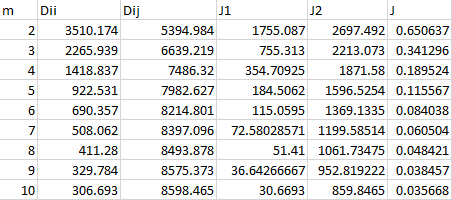
\includegraphics[width=.6\linewidth]{excel-table}
    \caption{Расчет численного показателя меры качества классификации}
    \label{fig:excel-table}
\end{figure}

Значения данного показателя качества классификации представлено графически на
рис 4.  Для этого построена диаграмма, на которой по оси Х – количество
кластеров, по оси Y – значения показателя J.

\begin{figure}[H]
    \centering
    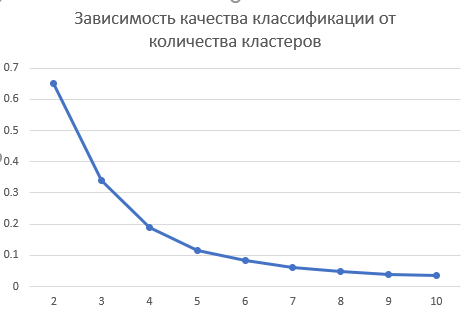
\includegraphics[width=.5\linewidth]{excel-graph}
    \caption{Диаграмма численной меры качества классификации}
    \label{fig:excel-graph}
\end{figure}

В соответствии с этим критерием оптимальным разбиением экспериментальных данных
является разбиение на 3 кластера.

\subsection{Иерархический анализ}
Был проведен иерархический анализ методом Уорда:

\begin{figure}[H]
    \centering
    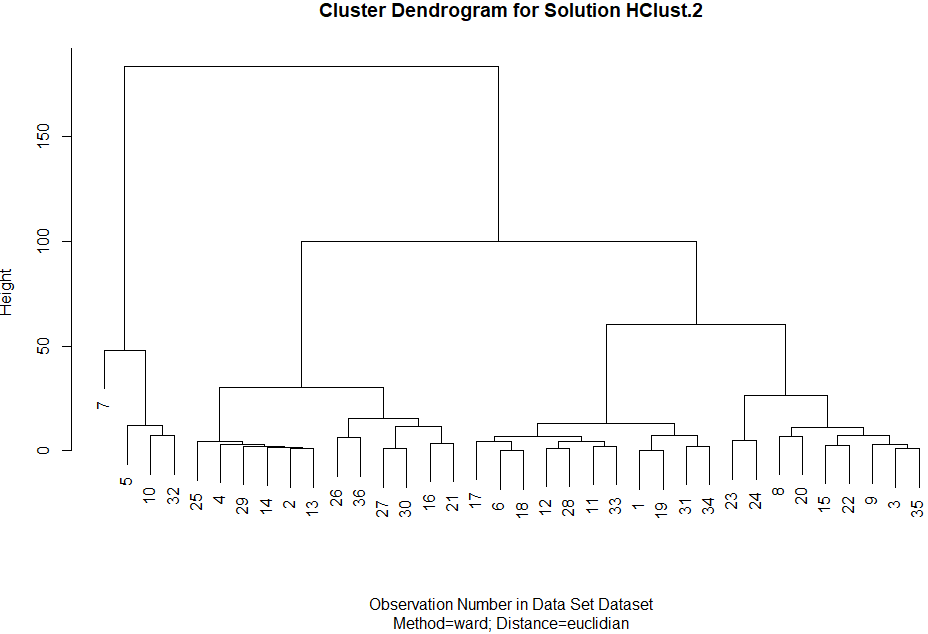
\includegraphics[width=\linewidth]{hierarchial-ward}
    \caption{Иерархический анализ методом Уорда}
    \label{fig:hierarchial-ward}
\end{figure}

Результатом анализа является количество элементов в каждом из кластеров:

\begin{lstlisting}
Rcmdr>  summary(as.factor(cutree(HClust.1, k = 3))) # Cluster Sizes
1  2  3 
16 14 20 
\end{lstlisting}
\pagebreak

Был проведен иерархический анализ методом простой связи:

\begin{figure}[H]
    \centering
    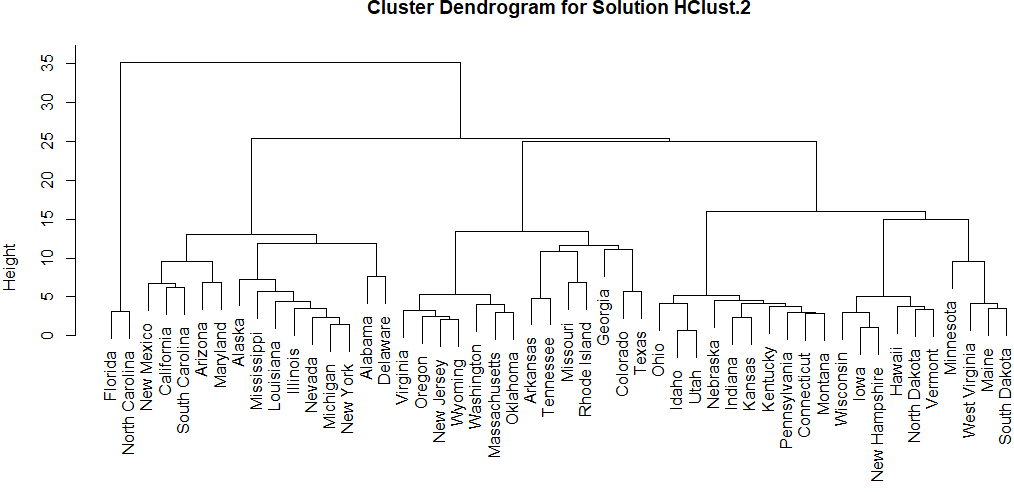
\includegraphics[width=\linewidth]{hierarchial-single-link}
    \caption{Иерархический анализ методом простой связи}
    \label{fig:hierarchial-single-link}
\end{figure}

Результатом анализа является количество элементов в каждом из кластеров:

\begin{lstlisting}
Rcmdr>  summary(as.factor(cutree(HClust.2, k = 3))) # Cluster Sizes
1  2  3 
14 34  2 
\end{lstlisting}

\section*{Выводы}
В ходе лабораторной работы провели многомерный анализ данных. Для этого
использовали кластеризацию, которая предназначена для разбиения совокупности
объектов на однородные группы (кластеры или классы). Если данные выборки
представить как точки в признаковом пространстве, то задача кластеризации
сводится к определению "сгущений точек". Целью кластеризации является поиск
существующих структур. Кластерный анализ позволяет сокращать размерность данных,
делать ее наглядной. Провели иерархический анализ с использованием k-средних.
Данный алгоритм является наиболее распространённым.

\end{document}